\documentclass{ximera}

\usepackage{microtype}
\usepackage{tikz}
\usepackage{tkz-euclide}
\usetkzobj{all}
\tikzstyle geometryDiagrams=[ultra thick,color=blue!50!black]

\renewcommand{\epsilon}{\varepsilon}



\title{Stereographic projection}
\begin{document}
\begin{abstract}
Here we start to develop another model for our geometry.
\end{abstract}
\maketitle


\subsection*{Stereographic projection coordinates}

Now we will examine the second way to produce coordinates uniformly for spherical, plane, and hyperbolic geometry that will allow us to pass smoothly through the three geometries.\\
Now let's project $K$-geometry,
\[
1=K\left(x^{2}+y^{2}\right)+z^{2} 
\]
onto the plane $z=1$ using the `South Pole' $S=(0,0,-1)$ as the center of
projection:
\begin{image}
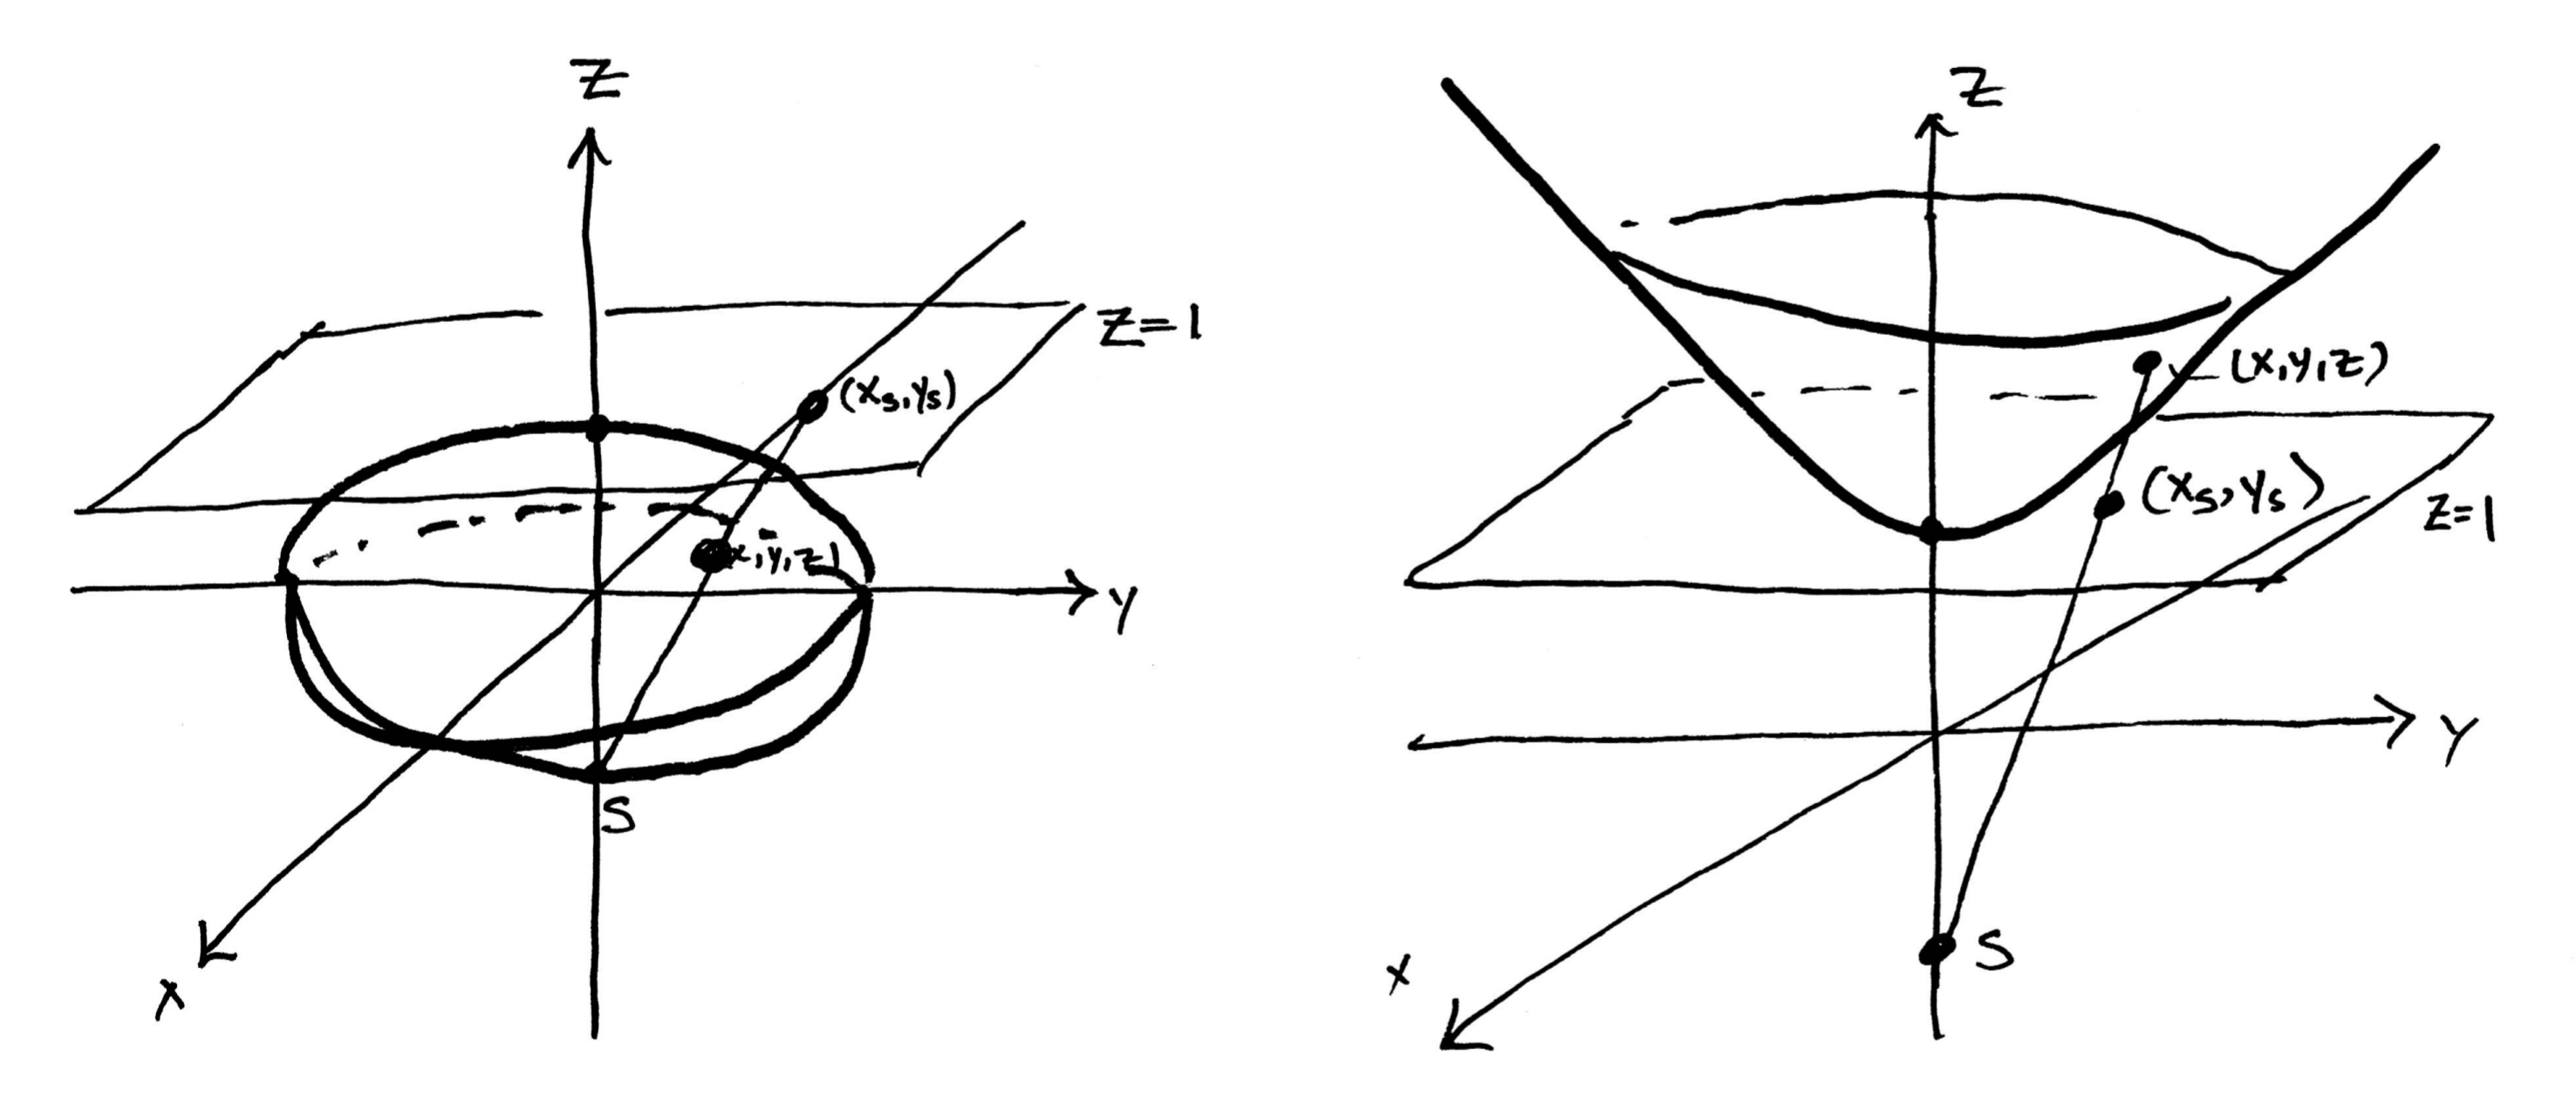
\includegraphics[width=5in]{stereoProj.png}
\end{image}
Let's look at this from a different vantage point, say with our eye
along the edge of the plane $z=1$:
\begin{image}
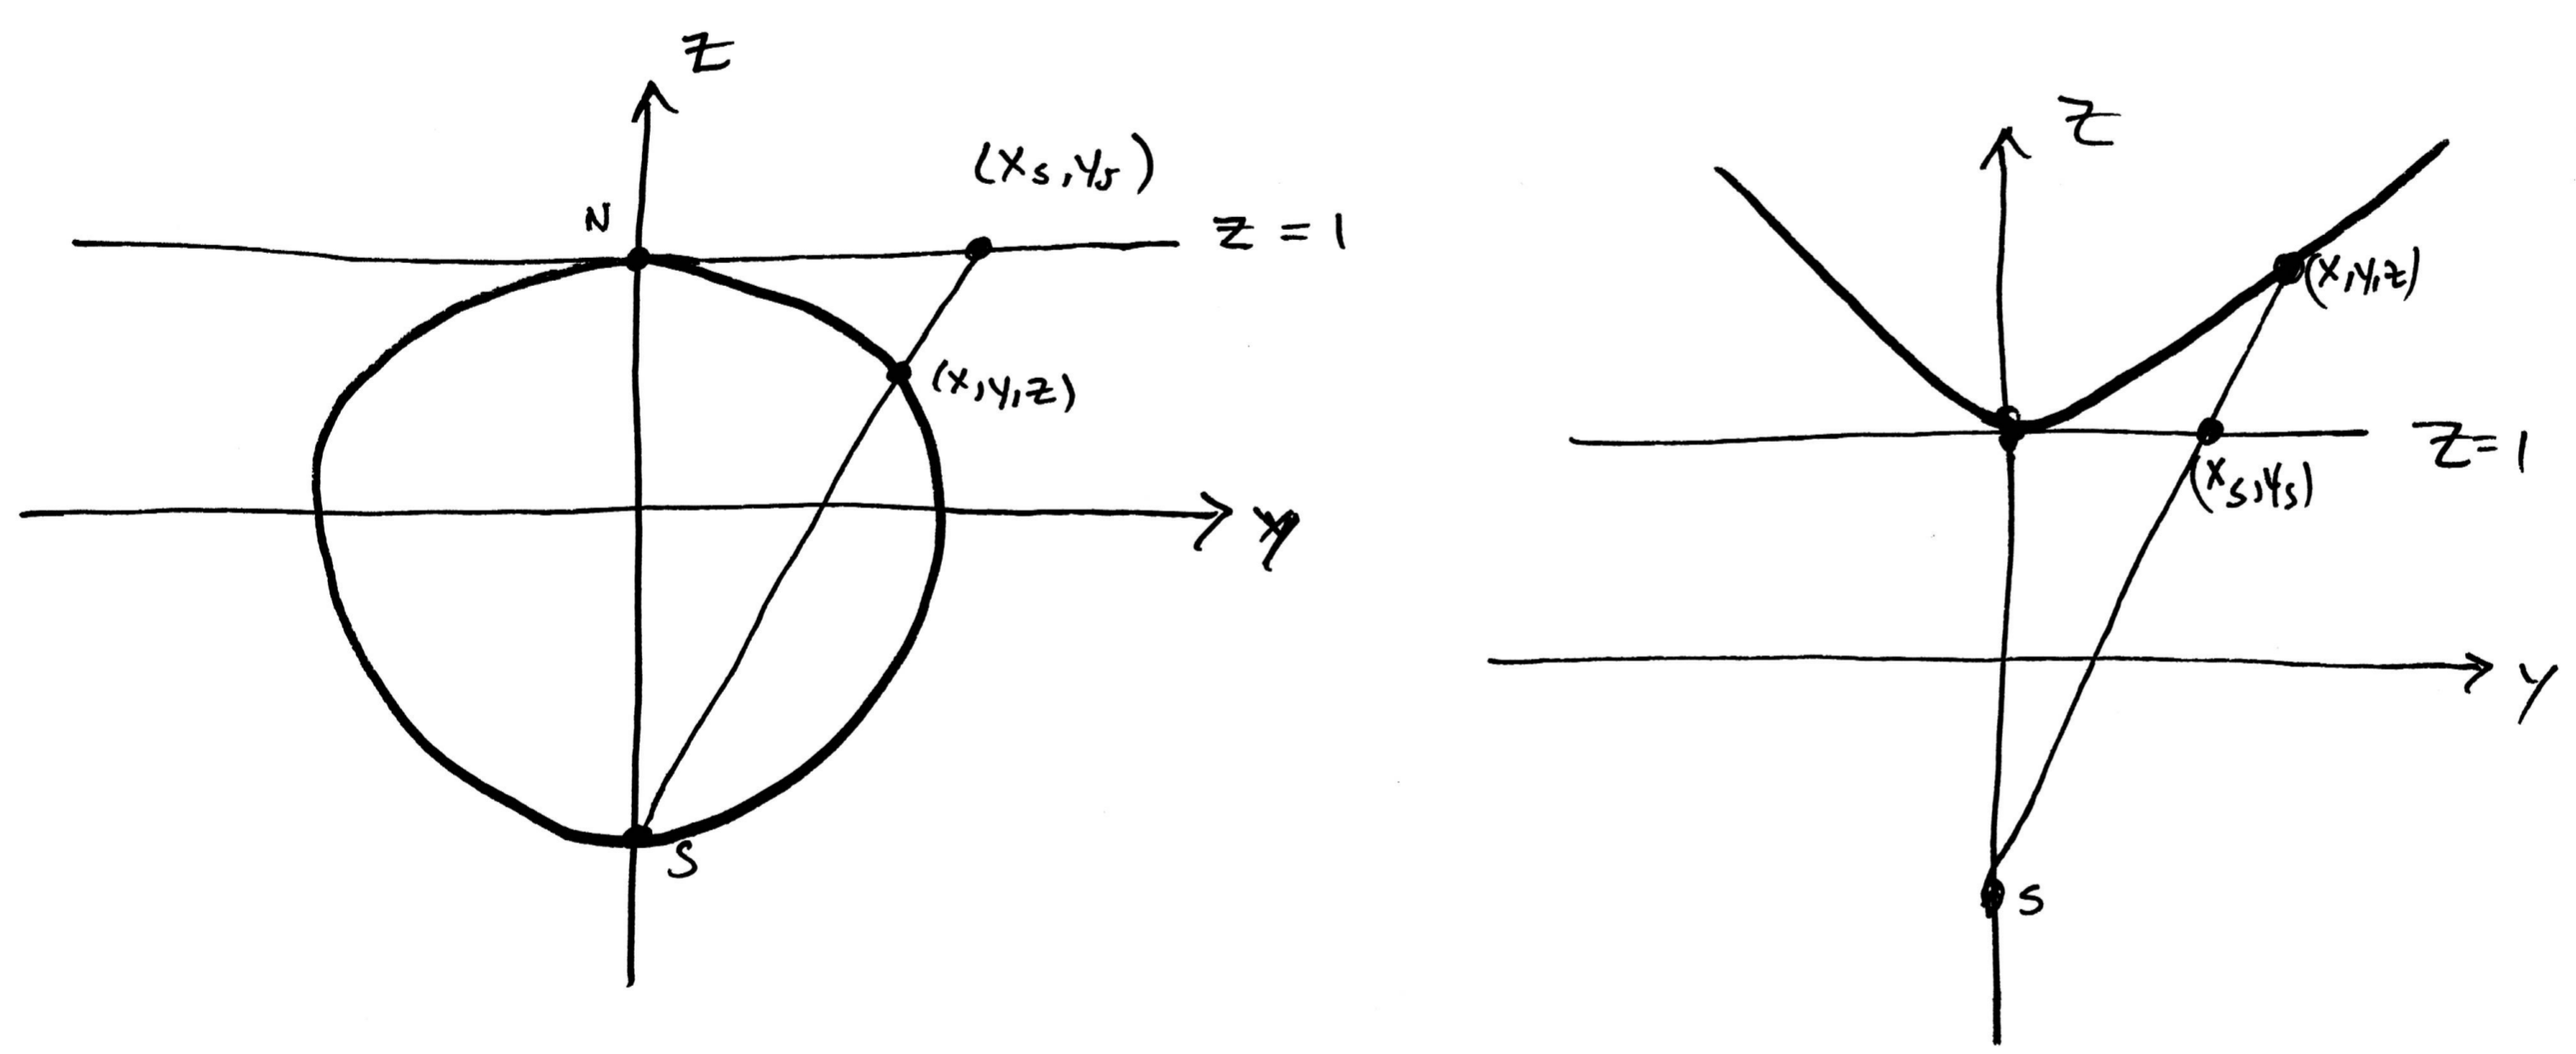
\includegraphics[width=5in]{stereoCross.png}
\end{image}

\begin{problem}
  If $K=1$ where does the `equator' map to? What about the `Northern hemisphere?' How about the `Southern hemisphere?'
  \begin{freeResponse}
    The `equator' maps to the circle of radius $2$ centered at the
    origin in the $(x_s,y_s)$ plane.  The `Northern hemisphere' maps
    inside this circle, and the `Southern hemisphere' maps outside the
    circle.
  \end{freeResponse}
\end{problem}

\begin{problem}
  Use similar triangles to explain why for any given $(x,y,z)$, there
  is a number $\rho$ such that
  \[
  \rho\cdot(x_s,y_s,2) = (x,y,z+1).
  \]
  \begin{freeResponse}
    Let $A = (x,y,z)$, $B= (x,y,-1)$, $A_s = (x_s,y_s,1)$ and
    $B_s=(x_s,y_s,-1)$. From the diagram above we see that
    \[
    \angle ASB = \angle A_s S B_s.
    \]
    Moreover, since $\triangle ASB$ and $\triangle A_s S B_s$ are
    right triangles, we now see that two of their angles have the same
    measure, and hence all three have the same measure. This means
    that these triangles are similar, and hence there they are
    dilations of one another. Hence there is a scale-factor $\rho$
    such that
    \[
    \rho\cdot(x_s,y_s,2) = (x,y,z+1).
    \]
  \end{freeResponse}
\end{problem}

\begin{problem}
  For the projection of the set $1=K\left(x^{2}+y^{2}\right)+z^{2}$
  onto the $z=1$ plane with center of projection $S$, write
  $(x_{s},y_{s})$ as a function of $(x,y,z)$.
  \begin{freeResponse}
    We know that
    \[
    \rho\cdot(x_{s},y_{s},2)=(x,y,z+1),
    \]
    hence $\rho=\frac{z+1}{2}$, and we may now write
    \begin{align*}
      x_{s} &=\frac{2x}{z+1},\\
      y_{s} &=\frac{2y}{z+1}.
    \end{align*}
  \end{freeResponse}
\end{problem}

\begin{problem}
  For the projection of the set $1=K\left(x^{2}+y^{2}\right)+z^{2}$
  onto the $z=1$ plane with center of projection $S$, write
  $(x,y,z)$ as a function of $(x_s,y_s)$.
  \begin{hint}
    Note that
      \[
      \rho\cdot(x_{s},y_{s},2)=(x,y,z+1) \qquad\text{and}\qquad z = 2\rho-1.
      \]
  \end{hint}
  \begin{hint}
    Hence if
    \[
    1 = K\left(x^2 + y^2\right) + z^2
    \]
    we may write
    \[
    1 = K\left((\rho\cdot x_s)^2 + (\rho\cdot y_s)^2\right) + (2\rho-1)^2
    \]
    and solve for $\rho$.
  \end{hint}
  \begin{freeResponse}
    This is slightly more complex than the previous problem; however,
    we will begin the same way. We know that
    \[
    \rho\cdot(x_{s},y_{s},2)=(x,y,z+1),
    \]
    hence $\rho=\frac{z+1}{2}$, and we may now write
    \begin{align*}
      x &= \rho \cdot x_s,\\
      y &= \rho \cdot y_s,\\
      z &= 2\rho-1.
    \end{align*}
    Now our task is to write $\rho$ in terms of $x_s$ and
    $y_s$. Using our assignments above, write
    \begin{align*}
      1 &= K\left(x^2 + y^2\right) + z^2\\
      1 &= K\left((\rho\cdot x_s)^2 + (\rho\cdot y_s)^2\right) + (2\rho-1)^2\\
      1 &= K\left((\rho\cdot x_s)^2 + (\rho\cdot y_s)^2\right) + 4\rho^2-4\rho + 1\\
    \end{align*}
    and so
    \begin{align*}
      0 &= K\left(\rho^2\cdot x_s^2 + \rho^2\cdot y_s^2\right) + 4\rho^2-4\rho\\
      0 &= \rho^2\cdot K\left(x_s^2 + y_s^2\right) + 4\rho^2-4\rho
    \end{align*}
    and since $\rho \ne 0$, we may write
    \begin{align*}
      \rho\cdot K\left(x_s^2 + y_s^2\right) + 4\rho-4 &=0 \\
      \rho\left(K\left(x_s^2 + y_s^2\right) + 4\right) &=4\\
      \rho &= \frac{4}{K\left(x_s^2 + y_s^2\right) + 4}.
    \end{align*}
    Hence
    \begin{align*}
      x &= \frac{4x_s}{K\left(x_s^2 + y_s^2\right) + 4},\\
      y &= \frac{4y_s}{K\left(x_s^2 + y_s^2\right) + 4},\\
      z &= \frac{4-K\left(x_s^2 + y_s^2\right)}{4+K\left(x_s^2 + y_s^2\right)}.\\
    \end{align*}
  \end{freeResponse}
\end{problem}


\section{Stereographic projection dot product}

Once more, we want to be able to find a dot product that will allow us
to compute lengths in stereographic projection coordinates that will agree
with the $K$-dot product, and hence the euclidean dot product.

\begin{problem}
Suppose we have a curve $X$ in $K$-warped space that is a function of
a curve $X_s$ in the plane $z=1$ space. So
\[
X_s(t) = \left( x_s(t),y_s(t)\right)
\]
and
\[
X(t) = 
\begin{cases}
  x(x_s(t),y_s(t)),\\
  y(x_s(t),y_s(t)),\\
  z(x_s(t),y_s(t)).
\end{cases}
\]
Use the chain rule to compute
\[
\dd[x]{t}, \qquad \dd[y]{t}, \qquad \dd[z]{t},
\]
in terms of $\dd[x_s]{t}$, $\dd[y_s]{t}$, $\pp[x]{x_s}$,
$\pp[y]{x_s}$, $\pp[z]{x_s}$, $\pp[x]{y_s}$, $\pp[y]{y_s}$,
and $\pp[z]{y_s}$.
  \begin{hint}
  Simply write down the answer from a previous problem with some minor
  changes.
  \end{hint}
  \begin{freeResponse}
  Write
  \begin{align*}
    \dd[x]{t} &= \begin{bmatrix}\pp[x]{x_s} & \pp[x]{y_s}\end{bmatrix}\cdot\begin{bmatrix}\dd[x_s]{t} & \dd[y_s]{t}\end{bmatrix}^\transpose = \pp[x]{x_s}\cdot\dd[x_s]{t}+\pp[x]{y_s}\cdot\dd[y_s]{t},   \\
    \dd[y]{t} &= \begin{bmatrix}\pp[y]{x_s} & \pp[y]{y_s}\end{bmatrix}\cdot\begin{bmatrix}\dd[x_s]{t} & \dd[y_s]{t}\end{bmatrix}^\transpose = \pp[y]{x_s}\cdot\dd[x_s]{t}+\pp[y]{y_s}\cdot\dd[y_s]{t},   \\
    \dd[z]{t} &= \begin{bmatrix}\pp[z]{x_s} & \pp[z]{y_s}\end{bmatrix}\cdot\begin{bmatrix}\dd[x_s]{t} & \dd[y_s]{t}\end{bmatrix}^\transpose = \pp[z]{x_s}\cdot\dd[x_s]{t}+\pp[z]{y_s}\cdot\dd[y_s]{t}.  
  \end{align*}
\end{freeResponse}
\end{problem}


\begin{problem}
  With the same setting as in the previous problem, rewrite the result
  of your computation in matrix notation to find $D_s$
  such that
\[
\begin{bmatrix}
\dd[x]{t} & \dd[y]{t} & \dd[z]{t}
\end{bmatrix}
=
\begin{bmatrix}
\frac{dx_s}{dt} & \frac{dy_s}{dt}
\end{bmatrix}\cdot D_s
\]
in terms of $\pp[x]{x_s}$, $\pp[y]{x_s}$, $\pp[z]{x_s}$,
$\pp[x]{y_s}$, $\pp[y]{y_s}$, and $\pp[z]{y_s}$.
\begin{hint}
  Simply write down the answer from a previous problem with some minor
  changes.
\end{hint}
\begin{freeResponse}
  \[
  D_s =
  \begin{bmatrix}
    \pp[x]{x_s} & \pp[y]{x_s} & \pp[z]{x_s} \\
    \pp[x]{y_s}   & \pp[y]{y_s}   & \pp[z]{y_s}
  \end{bmatrix}.
  \]
\end{freeResponse}
\end{problem}

\begin{problem}
  Now find $P_s$ in terms of $K$, $\pp[x]{x_s}$, $\pp[y]{x_s}$,
  $\pp[z]{x_s}$, $\pp[x]{y_s}$, $\pp[y]{y_s}$, and $\pp[z]{y_s}$ such
  that
  \[
  \left(\dd[x]{t}, \dd[y]{t}, \dd[z]{t}\right)\bullet_K
  \left(\dd[x]{t}, \dd[y]{t}, \dd[z]{t}\right)
  =
  \begin{bmatrix}
    \dd[x_s]{t} &  \dd[y_s]{t}
  \end{bmatrix}
  \cdot P_s
  \cdot
  \begin{bmatrix}
    \dd[x_s]{t} \\  \dd[y_s]{t}
  \end{bmatrix}.
  \]
  \begin{hint}
  Simply write down the answer from a previous problem with some minor
  changes.
  \end{hint}
  \begin{freeResponse}
    For completeness sake, we will include a complete solution.
    Working from the $K$-dot product, we need that
    \begin{align*}
    \left(\dd[x]{t}, \dd[y]{t}, \dd[z]{t}\right)\bullet_K
    \left(\dd[x]{t}, \dd[y]{t}, \dd[z]{t}\right)
    &=
    \begin{bmatrix}
      \dd[x]{t} & \dd[y]{t} & \dd[z]{t}
    \end{bmatrix}
    \begin{bmatrix}
      1 & 0 & 0\\
      0 & 1 & 0\\
      0 & 0 & K^{-1}
    \end{bmatrix}
    \begin{bmatrix}
      \dd[x]{t} \\ \dd[y]{t} \\ \dd[z]{t}
    \end{bmatrix}\\
    &=
    \begin{bmatrix}
      \frac{dx_s}{dt} & \frac{dy_s}{dt}
    \end{bmatrix}\cdot D_{s}\cdot
    \begin{bmatrix}
      1 & 0 & 0\\
      0 & 1 & 0\\
    0 & 0 & K^{-1}
    \end{bmatrix}
    \cdot
    \left(
    \begin{bmatrix}
      \frac{dx_s}{dt} & \frac{dy_s}{dt}
    \end{bmatrix}\cdot D_{s}
    \right)^\transpose\\
    &=
    \begin{bmatrix}
      \frac{dx_s}{dt} & \frac{dy_s}{dt}
    \end{bmatrix}\cdot D_{s}\cdot
    \begin{bmatrix}
      1 & 0 & 0\\
      0 & 1 & 0\\
    0 & 0 & K^{-1}
    \end{bmatrix}
    \cdot
    D_{s}^\transpose
    \cdot \begin{bmatrix}
      \frac{dx_s}{dt} \\ \frac{dy_s}{dt}
    \end{bmatrix}.
  \end{align*}
    Hence
    \begin{align*}
      P_s &=
      \begin{bmatrix}
        \pp[x]{x_s} & \pp[y]{x_s} & \pp[z]{x_s} \\
        \pp[x]{y_s} & \pp[y]{y_s} & \pp[z]{y_s}
      \end{bmatrix}
      \begin{bmatrix}
        1 & 0 & 0\\
        0 & 1 & 0\\
        0 & 0 & K^{-1}
      \end{bmatrix}
      \begin{bmatrix}
        \pp[x]{x_s} & \pp[x]{y_s}\\ 
        \pp[y]{x_s} & \pp[y]{y_s}\\
        \pp[z]{x_s} & \pp[z]{y_s}
      \end{bmatrix}\\
      &=
      \begin{bmatrix}
        \left(\pp[x]{x_s}\right)^2 + \left(\pp[y]{x_s}\right)^2 + \left(\pp[z]{x_s}\right)^2K^{-1} & \pp[x]{x_s}\pp[x]{y_s} + \pp[y]{x_s}\pp[y]{y_s} + \pp[z]{x_s}\pp[z]{y_s} K^{-1}\\
        \pp[x]{x_s}\pp[x]{y_s} + \pp[y]{x_s}\pp[y]{y_s} + \pp[z]{x_s}\pp[z]{y_s} K^{-1}       & \left(\pp[x]{y_s}\right)^2 + \left(\pp[y]{y_s}\right)^2 + \left(\pp[z]{y_s}\right)^2K^{-1}
      \end{bmatrix}.
    \end{align*}
  \end{freeResponse}
\end{problem}


Before we actually compute $P_s$, it will help to compute the partial
derivatives.


\begin{problem}
  Set
  \begin{align*}
    x(x_s,y_s) &=\rho\cdot x_s,\\
    y(x_s,y_s) &=\rho\cdot y_s,\\
    z(x_s,y_s) &=2\rho-1,
  \end{align*}
  and show that
  \[
  \begin{split}
    \pp[x]{x_s} &=\rho-\left(\frac{K}{2}\right)\rho^2x_s^2,\\
    \pp[y]{x_s} &=-\left(\frac{K}{2}\right)\rho^2x_sy_s,\\
    \pp[z]{x_s} &=-K\rho^2x_s,
  \end{split}
  \qquad
  \begin{split}
    \pp[x]{y_s} &= -\left(\frac{K}{2}\right)\rho^2x_sy_s,\\
    \pp[y]{y_s} &=\rho-\left(\frac{K}{2}\right)\rho^2y_s^2,\\
    \pp[z]{y_s} &= -K\rho^2y_s.
  \end{split}
  \]
  \begin{hint}
  Work in the following way:
  \begin{enumerate}
  \item Recall $x = \rho\cdot x_s$.
  \item Note that $\pp[x]{x_s} = \rho + x_s \cdot \pp[\rho]{x_s}$.
  \item Express the partial derivative in terms of $\rho$, $K$, $x_s$,
      and $y_s$.
  \end{enumerate}
  \end{hint}
  \begin{freeResponse}
    Write
    \begin{align*}
      \pp[x]{x_s} &= \rho + x_s\cdot \pp[\rho]{x_s}\\
      &= \rho + x_s\cdot \pp{x_s}\left(\frac{4}{K\left(x_s^2 + y_s^2\right) + 4}\right)\\
      &= \rho - x_s\cdot \left(\frac{4}{\left(K\left(x_s^2 + y_s^2\right) + 4\right)^{2}}\right)\cdot2Kx_s \\
      &=\rho-\left(\frac{K}{2}\right)\rho^2x_s^2.
    \end{align*}
    Similarly,
      \begin{align*}
      \pp[y]{x_s} &= y_s\cdot \pp[\rho]{x_s}\\
      &= y_s\cdot \pp{x_s}\left(\frac{4}{K\left(x_s^2 + y_s^2\right) + 4}\right)\\
      &= - y_s\cdot \left(\frac{4}{\left(K\left(x_s^2 + y_s^2\right) + 4\right)^{2}}\right)\cdot2Kx_s \\
      &= -\left(\frac{K}{2}\right)\rho^2x_sy_s.
      \end{align*}
      Finally,
      \begin{align*}
      \pp[z]{x_s} &= 2\cdot\pp[\rho]{x_s}\\
      &= 2\cdot\cdot \pp{x_s}\left(\frac{4}{K\left(x_s^2 + y_s^2\right) + 4}\right)\\
      &= - 2\cdot \left(\frac{4}{\left(K\left(x_s^2 + y_s^2\right) + 4\right)^{2}}\right)\cdot2Kx_s \\
      &= -\frac{K}\rho^2x_s.
      \end{align*}
      Now with entirely similar computations, we see
      \begin{align*}
        \pp[x]{y_s} &= -\left(\frac{K}{2}\right)\rho^2x_sy_s,\\
        \pp[y]{y_s} &=\rho-\left(\frac{K}{2}\right)\rho^2y_s^2,\\
        \pp[z]{y_s} &= -K\rho^2y_s.       
      \end{align*}
  \end{freeResponse}
\end{problem}


\begin{problem}
With the same setting as above, show that $P_s$ is
  \[
  P_s =
  \begin{bmatrix}
    \rho^2 & 0\\
    0 & \rho^2
  \end{bmatrix}.
  \]
  \begin{hint}
  When simplifying, combine the terms with the highest degree of $\rho$
  and note that
  \[
  \rho^{-1} = \frac{K\left(x_s^2 + y_s^2\right)+4}{4}.
  \]
\end{hint}
\begin{freeResponse}
  Write $\left(\pp[x]{x_s}\right)^2 + \left(\pp[y]{x_s}\right)^2 +\left(\pp[z]{x_s}\right)^2K^{-1}$
  \begin{align*}
    &=\left(\rho-\left(\frac{K}{2}\right)\rho^2x_s^2\right)^2 + \left(-\left(\frac{K}{2}\right)\rho^2x_sy_s\right)^2 +\left(-K\rho^2x_s\right)^2K^{-1}\\
    &=\rho^2 -K\rho^3x_s^2 + \left(\frac{K^2}{4}\right)\rho^4x_s^4 + \left(\frac{K^2}{4}\right)\rho^4x_s^2y_s^2 + K\rho^4x_s^2\\
    &=\rho^2 -K\rho^3x_s^2 + K\rho^4x_s\left(\left(\frac{K}{4}\right)x_s^4 + \left(\frac{K}{4}\right)y_s^2 + 1\right)\\
    &=\rho^2 -K\rho^3x_s^2 + K\rho^4x_s\left(\frac{K\left(x_s^2+y_s^2\right)+4}{4}\right)\\
    &=\rho^2 -K\rho^3x_s^2 + K\rho^4x_s\rho^{-1}\\
    &=\rho^2.
  \end{align*}
  That $\pp[x]{x_s}\pp[x]{y_s} + \pp[y]{x_s}\pp[y]{y_s} + \pp[z]{x_s}\pp[z]{y_s} K^{-1}$
  \begin{align*}
    &=\left(\rho-\left(\frac{K}{2}\right)\rho^2x_s^2\right)\left(-\left(\frac{K}{2}\right)\rho^2x_sy_s\right)
    + \left(-\left(\frac{K}{2}\right)\rho^2x_sy_s\right)\left(\rho-\left(\frac{K}{2}\right)\rho^2y_s^2\right)
    + \left(-K\rho^2x_s\right)\left(-K\rho^2y_s\right) K^{-1}\\
    &=
    -\left(\frac{K}{2}\right)\rho^3x_sy_s+\left(\frac{K^2}{4}\right)\rho^4x_s^3y_s
    -\left(\frac{K}{2}\right)\rho^3x_sy_s+\left(\frac{K^2}{4}\right)\rho^4x_sy_s^3
    + K\rho^4 x_sy_s\\
    &= -K\rho^3x_sy_s + K\rho^4x_sy_s\left(\frac{K\left(x_s^2+y_s^2\right)+4}{4}\right)\\
    &= -K\rho^3x_sy_s + K\rho^4x_sy_s\rho^{-1}\\
    &= -K\rho^3x_sy_s + K\rho^3x_sy_s\\
    &=0.
  \end{align*}
  With entirely analogous computations, we see that 
    \[
    P_s =
    \begin{bmatrix}
      \rho^2 & 0\\
      0 & \rho^2
    \end{bmatrix}.
    \]
\end{freeResponse}
\end{problem}

\begin{definition}
  Let $V_s$ and $W_s$ be a vectors in $(x_s,y_s)$-coordinates
  originating at the same $(x_s,y_s)$-coordinate. Define
  \[
  V_s \bullet_s W_s = V_s \cdot P_s \cdot W_s^\transpose
  \]
  where
  \[
  P_s =
  \begin{bmatrix}
    \rho^2 & 0\\
    0 & \rho^2
  \end{bmatrix}
  \]
  is determined by the coordinate that the vectors originate from.
\end{definition}








\section{Again, when the finite is infinite and the infinite is finite}

Just like central projection, stereographic projection allows us to
think about both ``finite'' areas and ``infinite'' areas in new ways.

\paragraph{When $K$ is positive, the finite is infinite}

When $K>0$, we are working with a sphere. As we know, a sphere has
finite surface area.



\begin{problem}
  Where does the Northeren hemisphere of the $R$-sphere map to under stereographic projection?
  \begin{hint}
    A picture is worth a thousand words!
  \end{hint}
  \begin{freeResponse}
  \end{freeResponse}
\end{problem}


\begin{problem}
  Where does the Southeren hemisphere of the $R$-sphere map to under stereographic projection?
  \begin{hint}
    A picture is worth a thousand words!
  \end{hint}
  \begin{freeResponse}
  \end{freeResponse}
\end{problem}


\begin{problem}
  As a point approaches the South Pole of the $R$-sphere where does it
  move to under stereographic projection?
  \begin{hint}
    Simply transform the relevant coordinate.
  \end{hint}
  \begin{freeResponse}
  \end{freeResponse}
\end{problem}



\begin{problem}
  Explain why one might say that stereographic projection makes the
  ``finite'' seem ``infinite.''
    \begin{freeResponse}
    \end{freeResponse}
\end{problem}




\paragraph{When $K$ is negative, the infinite is finite}


Notice that, if $K<0$, the equation of $K$-geometry becomes
\[
z^{2}-|K|\left(x^{2}+y^{2}\right)  =1.
\]
This describes a $K$-geometry forms a $2$-sheeted hyperboloid with the
$z$-axis as major axis. We will only consider the sheet on which $z$
is positive as forming the $K$-geometry.  Of critical importance, note

\begin{center}
  \textbf{this hyperboloid has infinite surface area.}
\end{center}

The hyperboloid above is obtained by rotating the hyperbola
\[
z^{2}-\left\vert K\right\vert x^{2}= 1
\]
in the $(x,z)$-plane around the $z$-axis.



\begin{problem}
  Assume we have a point in $K$-geometry that is shooting off to
  infinity. What is the maximum distance the image of this point can
  be from the origin in stereographic projection?
  \begin{hint}
    First rewrite $z^{2}-|K|x^{2} =1$ as
    \[
    z = \sqrt{1+|K|x^2}
    \]
    and explain why this is acceptable.
  \end{hint}
  \begin{hint}
    Explain why computing this limit
    \[
    \lim_{x\to \infty} \frac{\sqrt{1+|K|x^2}}{x}
    \]
    helps us in this context.
  \end{hint}
  \begin{freeResponse}
    Since we are only considering the upper hyperboloid, we need only
    look at the upper hyperbola. Hence we may look at
     \[
    z = \sqrt{1+|K|x^2}.
    \]
    To compute the maximum distance the image of a point can be from
    the origin, look at 
    \[
    \lim_{x\to \infty} \frac{\sqrt{1+|K|x^2}}{x}
    \]
    as this computes the ``end-behavior'' of the ``slope'' of the
    curve. Write
    \begin{align*}
      \lim_{x\to \infty} \frac{\sqrt{1+|K|x^2}}{x} &= \lim_{x\to \infty} \frac{\sqrt{1+|K|x^2}}{x}\cdot \frac{1/x}{1/x}\\
      &= \lim_{x\to \infty} \sqrt{1/x^2+|K|}\\
      &= \sqrt{|K|}.
    \end{align*}
    Hence one projection is given by $z = x\sqrt{|K|}-1$.
  \end{freeResponse}
\end{problem}


Rotating the line found above gives the ``asymptotic cone.'' The
stereographic projection coordinates $(x_{s},y_{s})$ of $K$-geometry
when $K<0$ only correspond to points in $K$-geometry when
$(x_{s},y_{s},1)$ lies \textit{inside} the asymptotic cone.

\begin{problem}
  When $K<0$, find the radius of the disk in the plane $z=1$ whose
  perimeter is determined by the asymptotic cone. 
  \begin{hint}
    Work with the asymptote(s) you found above.
  \end{hint}
  \begin{freeResponse}
    We must find where $z = x\sqrt{|K|}-1$ intersects the line $z=1$. To do this, simply solve
    \[
    1 = x\sqrt{|K|}-1
    \]
    for $x$, and so the radius is $2/\sqrt{|K|}$.
  \end{freeResponse}
\end{problem}

\begin{problem}
  Explain why one might say that stereographic projection makes the
  ``infinite'' seem ``finite.''
    \begin{freeResponse}
    \end{freeResponse}
\end{problem}

The $(x_{s},y_{s})$-coordinates are called \dfn{Poincar\'e
  coordinates} for hyperbolic geometry and the disk of radius
$2/\sqrt{|K|}$ called the \dfn{Poincar\'e model} for hyperbolic
geometry in honor of the famous French geometer, Henri Poincar\'e.









\begin{problem}
Summarize the results from this section. In particular, indicate which
results follow from the others.
\begin{freeResponse}
\end{freeResponse}
\end{problem}


\end{document}
